\section{Entwicklungsprozess}

\subsection{Beschaffung von 3D-Modellen}
Die bereits in der Projektarbeit entwickelte Basis des Frameworks erlaubt
die Erstellung von geometrischen Formen \doublecite[15]{philipp}. 
Dafür wird im Backend die Rendering-API pythreejs verwendet.
Diese bietet anhand von vorgefertigten Klassen wie BoxGeometry und CylinderGeometry eine einfache
Möglichkeit primitive Geometrien zu erstellen und zu rendern \doublecite{pythreejs_Geometry_types}.
Für die Erstellung von komplexen und individuellen Geometrien, wie die eines Industrieroboters oder dessen Glieder,
bietet pythreejs die Klasse BufferGeometry, welche expliziet mit den Vertices, Indices und Normals
eines Mesh-Modells initialisiert werden kann \doublecite[]{pythreejs_doc}. Diese Daten können entweder aus bestehenden 3D-Dateien
(z.B .stl, .obj, .dae) extrahiert oder durch eigene Verfahren erzeugt werden.

Im Framework soll nicht ein einziges Mesh-Modell des vollständigen Roboters geladen werden,
da sich dessen Gelenke in diesem Fall nicht unabhängig voneinander animieren ließen.
Stattdessen muss das 3D-Modell des Roboters aus mehreren separaten Meshes bestehen,
die jeweils ein einzelnes Glied (Link) repräsentieren.
Diese Glieder werden anschließend entsprechend ihrer Positionen und Transformationen innerhalb der kinematischen Kette zusammengesetzt.

Da es im Internet viele 3D-Modelle von Industrierobotern in Form solcher 3D-Dateien gibt,
war der erste Schritt zur Erweiterung des Frameworks die Recherche nach geeigneten Quellen solcher Modelle.
Die Recherche ergab folgende Ergebnisse:

\vspace{1em}
\begin{table}[H]
\centering
\begin{tabular}{|p{4cm}|p{5.5cm}|p{4cm}|}
\hline
\textbf{Quelle} & \textbf{Beschreibung} & \textbf{Dateiformate} \\
\hline
ROS-Industrial & Offizielle Roboterbeschreibungen für MoveIt/ROS & URDF, STL, DAE \\
\hline
GrabCAD & CAD-Bibliothek mit vielen industriellen Modellen & STL, STEP, SLDASM \\
\hline
Thingiverse & Plattform für 3D-druckbare Modelle & STL, OBJ \\
\hline
Onshape Public Library & Online-CAD-Modelle mit direktem Export & beliebig \\
\hline
Peter Corke Robotics Toolbox & Kinematik- und Modellbibliothek für Lehre und Forschung & URDF, STL \\
\hline
\end{tabular}
\caption{Online-Quellen für 3D-Robotermodelle}
\label{tab:robotermodelle}
\end{table}
\vspace{1em}

ROS-Industrial ist ein Open-Source-Projekt welches Module und Ressourcen bereitstellt die innerhalb des ROS-Ökosystems genutzt werden können.
Dabei werden diese Ressourcen sowohl von der Community genutzt wie auch gewartet und sind komplett Quelloffen.
Viele dieser Ressourcen können unter Github von ROS-Industrial runtergeladen werden \doublecite[]{ROS_Industrial}.
Zu diesen Ressourcen zählen auch 3D-Modelle von Industrierobotern die unter dem Github-Topic moveit gefunden werden können.
Dort finden sich zahlreiche Repositories,
die jeweils die Roboterbeschreibungen eines bestimmten Herstellers enthalten \doublecite[]{ROS_Industrial_repo_search}.
Diese Repositories sind in der Regel als eigenständige ROS-Packages organisiert und enthalten häufig
weitere Unterpackages für die einzelnen Robotermodelle.
Dies entspricht der typischen Struktur innerhalb des ROS-Ökosystems,
in dem Software, Konfigurationen und Modelle modular in Form von ROS-Packages aufgebaut sind \doublecite[]{ROS_Packages_Design}.
Die Unterpackages enthalten zudem Dateien im Xacro Format, wobei es sich um die URDF-Beschreibung des jeweiligen Modells handelt.

Eine weitere Quelle für 3D-Modelle von Industrierobotern ist GrabCAD, ein Unternehmen,
das Softwarelösungen im Bereich 3D-Druck anbietet.
Darüber hinaus betreibt GrabCAD eine Online-Plattform,
auf der Mitglieder der Community CAD-Dateien hochladen, teilen und herunterladen können \doublecite[]{GrabCAD_Company}.
Auf der Online-Plattfrom sind CAD-Dateien von Industrierobotern wie zum Beispiel der kr\_140\_3200\_2 von KUKA, der
der PUMA 560 und viele andere.
Die CAD-Dateien liegen in den meisten Fällen im STEP, STL oder im SLDASM Format vor und lassen sich mit CAD-Software
wie beispielsweise FreeCAD öffnen und bearbeiten.


Weiterhin ist Thingiverse eine Quelle für 3D-Modelle von Industrierobotern.
Ähnlich wie bei der Online-Plattform von GrabCAD handelt es sich bei Thingiverse
ebenfalls um eine solche Plattform die von Ultimaker betrieben wird.
Auch bei dieser Plattform gibt es zahlreiche CAD-Dateien von Industrierobotern
die von der Community geteilt werden, wobei der Fokus eher auf dem 3D-Druck liegt \doublecite[]{Thingiverse}.


Bei Onshape handelt es sich um eine browserbasierte CAD-Software,
die als browserbasierte Software-as-a-Service Lösung von dem Unternehmen PTC bereitgestellt wird.
Als Nutzer der Plattform ist es möglich Repositories in der Cloud anzulegen und diese mit anderen Nutzern zu teilen \doublecite[]{onShape}.
Hier befinden sich zahlreiche Repositories aus denen 3D-Modelle von Industrierobotern in einem beliebigen Format herunterladen werden können.


Abschließend wurde versucht die 3D-Modelle aus der Robotics-Toolbox von Peter Corke zu extrahieren,
welche von Github oder über pip herunterladen und installiert werden kann.
Die Toolbox bietet zahlreiche Funktionen für die Modellierung und Analyse robotischer Systeme und erlaubt
die visuelle Simulation von Robotern innerhalb eines eigenen Renderers namens Swift \doublecite[77]{Robotics_Vision_and_Control}.
Die dafür benötigten 3D-Modelle werden bei der Installation der Toolbox mitgeliefert und befinden sich samt einer URDF-Beschreibung
im Verzeichnis ./robotics-toolbox-python/rtb-data/rtbdata/xacro.

Die genannten Quellen stellen eine geeignete Möglichkeit zur Beschaffung der 3D-Modelle dar.
Da es innerhalb des Frameworks auch möglich sein soll die Bewegung der Roboter zu simulieren,
werden weitere Informationen wie die Position und Orientierung von Gelenken und Gliedern,
Hierarchien innerhalb der kinematischen Kette sowie Minimal- und Maximal-Grenze der Gelenke benötigt.
Diese Informationen liegen üblicherweise im URDF-Format vor.
Obwohl es grundsätzlich möglich ist, diese Informationen manuell zu rekonstruieren und in das URDF-Format zu übertragen,
ist dies mit erheblichem Aufwand verbunden.
Daher sind Quellen, die neben den 3D-Modellen bereits eine vollständige URDF-Beschreibung bereitstellen, von besonderem Vorteil.
von den genannten Quellen stellen nur ROS-Industrial und die Robotics-Toolbox von Peter Corke solche URDF-Beschreibungen zur verfügung.
Darüber hinaus ist die Anzahl der Dreiecke in den Meshes dieser beiden Quellen bereits reduziert, was die Ladezeit verbessert.
Aus diesen Gründen sind im weiteren Verlauf des Entwicklungsprozesses hauptsächlich diese beiden Quellen verwendet worden.



\subsection{Laden von 3D-Modellen}
Um die 3D-Modelle der Industrieroboter innerhalb des Frameworks rendern zu können,
müssen diese zunächst aus den heruntergeladenen Dateien in den Arbeitsspeicher geladen werden.
Hierfür wird die Python-Bibliothek trimesh verwendet, die das Einlesen und die Verarbeitung von triangulären Meshes unterstützt.
Die Bibliothek erlaubt das Laden gängiger Formate wie STL, OBJ, DAE und weiterer \doublecite[]{trimesh}.
Die geladenen Roboter bestehen dabei nicht aus einer einzigen Mesh,
sondern setzen sich aus mehreren einzelnen Teil-Meshes zusammen, von denen jede durch eine eigene Datei (.stl, .obj, .dae) repräsentiert wird.
Diese Teilmodelle entsprechen den physischen Gliedern des Roboters.
Beim Laden der Meshes ist aufgefallen dass der Vorgang pro Mesh einige Sekunden in Anspruch nimmt und Insbesondere bei komplexeren Modellen
zu einer Gesamtladezeit von knapp einer Minute pro Roboter-Modell geführt hat.
Verwendet wurde eine Intel\textsuperscript{\textregistered} Core\texttrademark\ i7-9700K CPU mit 3,60\,GHz, 8 Kernen und 8 logischen Prozessoren.
Um die Ladezeiten der Meshes zu reduzieren und dadurch die Benutzerfreundlichkeit zu verbessern, wurde das NPZ-Format von NumPy verwendet.
Im Gegensatz zu den üblichen Text-basierten Formaten handelt es sich beim NPZ-Format um ein binäres Format,
welches maschinell effizienter eingelesen werden kann \doublecite[]{numpy_npy_npz_format}.
Die 3D-Modelle wurden in das NPZ-Format konvertiert, um die Ladezeiten zu optimieren.
Um die Auswirkung auf die Ladezeit nachzuvollziehen wurde eine Messung durchgeführt.
Dabei wurde die Ladezeit beim Einlesen einer .npz-Datei mit derjenigen beim Laden der entsprechenden .stl-Datei für dieselbe Mesh verglichen.
Der Test, welcher dieser Arbeit unter dem Namen benchmark\_npz\_vs\_stl.ipynb beiliegt zeigt, dass der Ladevorgang aus der .stl Datei
c.a 0.7757 Sekunden benötigte. Der Ladevorgang aus der .npz-Datei benötigte hingegen c.a 0.0002 Sekunden und ist damit c.a 2800 mal schneller:

\begin{center}
    \begin{verbatim}
    Ausführungszeit-STL: 0.775746 Sekunden für 570279 Faces
    Ausführungszeit-NPZ: 0.000276 Sekunden für 570279 Faces
    \end{verbatim}
\end{center}

Für diesen Test ist die bereits erwähnte Intel\textsuperscript{\textregistered} Core\texttrademark\ i7-9700K CPU mit 3,60\,GHz, 8 Kernen und 8 logischen Prozessoren zum Einsatz gekommen.
Um das NPZ-Format nutzen zu können, müssen die 3D-Modelle zunächst in dieses Format konvertiert und dauerhaft gespeichert werden.
So können sie beim nächsten Start des Frameworks direkt aus der .npz-Datei geladen werden.
Dafür wurde ein Lazy-Loading-Mechanismus implementiert, der zunächst prüft, ob bereits eine .npz-Datei für die gewünschte Mesh vorhanden ist.
Abhängig vom Ergebnis wird die Datei entweder geladen oder zunächst erstellt:

\vspace{1em}
    \begin{algorithm}
        \caption{Laden eines 3D-Modells aus einer NPZ-Datei}
        \begin{algorithmic}[1]
            \State \textbf{Input:} \textit{filepath}, \textit{filepath\_npz}
            \If{\textbf{not} \textit{is\_file(filepath\_npz)}}
                \State \textit{to\_npz(filepath, filepath\_npz)}
            \EndIf
            \State \Return \textit{load\_from\_npz(filepath\_npz)}
        \end{algorithmic}
    \end{algorithm}
\vspace{1em}












\subsection{Graphische Darstellung von Industrierobotern}

Die geladenen Daten werden anschließend in BufferGeometry-Objekte überführt, wie sie von pythreejs benötigt werden, 
um als Bestandteil einer Szene gerendert werden zu können. 
Bereits in der vorangegangenen Projektarbeit wurde hierfür eine Klasse namens Environment entwickelt, 
die die Erstellung einer Szene einschließlich Beleuchtung, Kamera, Basiskoordinatensystem und Gitter kapselt. 
Darüber hinaus verwaltet sie alle Objekte, die über die display-Funktion im Jupyter Notebook gerendert werden sollen \doublecite[15]{philipp}.
Diese Objekte erben von der Klasse Object3D aus pythreejs und können ihrerseits weitere Object3D-Instanzen über ein Array namens children enthalten. 
Transformationen werden dabei an die children weitergegeben, wodurch Transformationshierarchien entstehen. 
Dieses Prinzip lässt sich gezielt für die visuelle Darstellung und Animation von Robotern mit serieller Kinematik nutzen: 
Jedes Glied der kinematischen Kette verwaltet dabei das nachfolgende Gelenk als child, welches wiederum das nächste Glied als child verwaltet. 
Auf diese Weise bewegen sich alle nachfolgenden Glieder korrekt mit, wenn ein vorheriges Glied transformiert wird.

In den meisten stl-, obj- und dae-Dateien werden wenn überhaupt nur die Vertex-Normalen gespeichert.
Damit die Oberflächen des gerenderten Roboters glatt erscheinen, muss das

Die folgende Abbildung zeigt die mit dem Framework gerenderten Einzelglieder des KR6 R900-2 von KUKA.

\vspace{1em}
\begin{figure}[H]
    \centering
    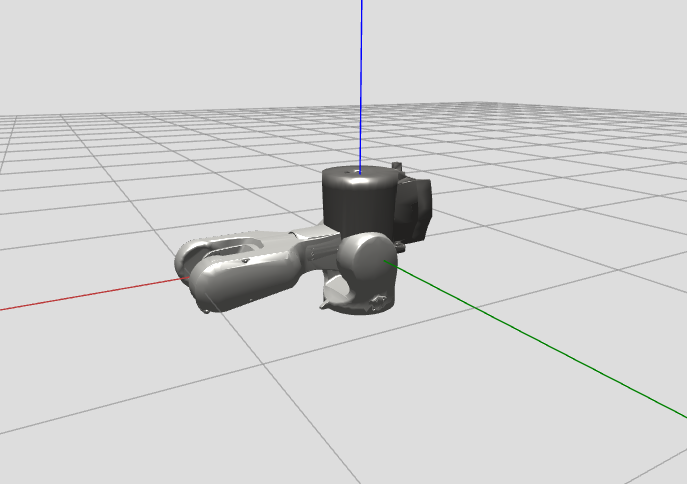
\includegraphics[width=0.8\textwidth]{images/load_links.PNG}
    \caption{Ansicht der 3D-Szene des Frameworks mit einzelnen Gliedern des KR6 R900-2 von KUKA}
    \label{fig:render_links}
\end{figure}
\vspace{1em}

In dieser Darstellung besteht noch keine Hierarchie zwischen den einzelnen Gliedern. 
Alle Glieder sind im Ursprung des Basiskoordinatensystems positioniert und bilden daher noch keine zusammenhängende Roboterstruktur. 
Um eine korrekte Darstellung zu erreichen, müssen die Glieder entsprechend einer URDF-Beschreibung räumlich korrekt positioniert und orientiert werden.

